\documentclass[12pt]{report}

% Include all packages from file.
\usepackage[english]{babel}
\usepackage[utf8]{inputenc}
\usepackage{amsmath}
\usepackage{csquotes}% Recommended

\usepackage[a4paper,width=150mm,top=25mm,bottom=25mm]{geometry} %Paper margins
\usepackage{tikz}
\usetikzlibrary{calc}
\newcommand\HRule{\rule{\textwidth}{1pt}}

\usepackage[nolist,nohyperlinks]{acronym}

\usepackage{newtxtext,newtxmath}

\usepackage[comma,colon]{natbib}
\bibliographystyle{agsm}

\usepackage{hyperref}






\renewcommand{\contentsname}{Table of Contents}
\renewcommand{\baselinestretch}{1.5}

% HEADER AND FOOTER--------------------------
\patchcmd{\chapter}{\thispagestyle{plain}}{\thispagestyle{fancy}}{}{}
\pagestyle{fancy}
\fancyhf{}
\lhead{\fontsize{10}{12}\leavevmode\selectfont\color{gray}{Lazy-Koala: A Lazy Approach for Root Cause Analysis in Distributed Systems}}
\rfoot{\fontsize{10}{12}\leavevmode\selectfont\color{gray}{\thepage}}
\lfoot{\fontsize{10}{12}\leavevmode\selectfont\color{gray}{Isala Piyarisi | 2018421}}
\renewcommand{\headrulewidth}{0pt}
% END HEADER AND FOOTER--------------------------


% Document begins here
\begin{document}

% TITLE PAGE---------------------------------------------------
\begin{titlepage}

\begin{tikzpicture}[remember picture, overlay]
  \draw[line width = 1pt] ($(current page.north west) + (1cm,-1cm)$) rectangle ($(current page.south east) + (-1cm,1cm)$);
\end{tikzpicture}

\begin{center}

% Upper part of the page
% \text{\large Informatics Institute of Technology}\\[0.1cm]
% \text{\large In Collaboration With}\\[0.5cm]
% \text{\large University of Westminster, UK}\\[2.5cm]

% Title

\includegraphics[width=5.0cm]{assets/IIT-Logo.png}\\[0.7cm]
{ \Huge Anomaly Detection \& Root Cause Analysis\\
In Distributed Systems }\\[0.7cm]
% \begin{minipage}{0.45\textwidth}
\text{\LARGE  Project Specifications Design and Prototype}\\[0.5cm]

% Authors
% \text{\large A dissertation by}\\[0.1cm]
\text{\large Isala Piyarisi}\\[0.1cm]
\text{\large w1742118 / 2018421}\\[3.2cm]

% Supervisor
\text{\large \textbf{Supervisor}: Guhanathan Poravi}\\[0.1cm]
\text{\large \textbf{Date}: $13^{rd} $ February 2022}\\[0.1cm]
\text{\large \textbf{Department}: Computer Science}\\[0.1cm]
\text{\large \textbf{Keywords}: Cloud Computing, AIOps, Monitoring, Disaster Recovery}\\[5cm]


\large{Submitted in partial fulfilment of the requirements for the \\
BSc(Hons) Computer Science degree at the \\
University of Westminster.
} \\[0.5cm]


\end{center}

\end{titlepage} 

% Page Numbering---------------------------------------------
\pagenumbering{roman}

\chapter*{Abstract}

Cloud computing has shown a considerable growth in the past few years, due to its scalability and convenience. With this change, a new programming paradigm called cloud-native was originated. Cloud-native applications are often developed as a set of stand-alone microservices yet could depend on each other to provide a unified experience. Although microservices introduce many benefits when it comes to flexibility and scalability, it could be a great affliction to operate in production. Specifically, when operating a large system with hundreds of microservices interacting with each other, even the smallest problem could result in failures throughout the system.

% Cloud computing is a steady rise for the past few years due to its scalability and ease of use. With this change, a new programming paradigm called cloud-native was born. Cloud-native applications are often developed as a set of stand-alone microservices yet, it could depend on each other to provide a unified experience. 

% This helps different teams to work on different services which increases the development velocity. This works well for medium to large companies but over time this mesh of services could become very complicated to a point where it's very difficult for a single person to understand the entire system. When the system consists of thousands of individual services talking and depending on each other, the network layer of that system becomes chaotic. A failure in a single point could create a ripple effect across the entire system. When something like that happens it could take a considerable amount of time to zero in on the exact point of the failure.

The foci of this project are twofold. First, the authors introduce a robust Kubernetes native toolkit that helps both researchers and developers collect and process service telemetry data with zero instrumentation. Secondly, the authors proposed a novel way to detect anomalies by encoding raw metric data into an image-like structure and using a convolutional autoencoder to acquire the knowledge of the general data distribution for each service and to detect outliers. Finally, a directed graph was used along with anomaly scores calculated prior were used to visually show the spread of an anomaly to the user. 

After an extensive testing and evaluation process it was found out that the telemetry extraction components are both resilient and lightweight even under sustained load, while the anomaly prediction algorithm is accurate and generalizable. 
\newline
\newline
\textbf{Keywords}:
AIOps, Monitoring, Disaster Recovery, eBPF, Kubernetes
\newline
\textbf{Subject Descriptors}:
• Computing methodologies $\rightarrow$ Machine learning $\rightarrow$ Learning paradigms $\rightarrow$ Unsupervised learning $\rightarrow$ Anomaly detection • Computer systems organization $\rightarrow$ Architectures $\rightarrow$ Distributed architectures $\rightarrow$ Cloud computing
\addcontentsline{toc}{chapter}{Abstract}

% Table of Contents---------------------------------------------------
\tableofcontents
% List of Figures---------------------------------------------------
% \cleardoublepage
{\let\clearpage\relax
\listoffigures
}
\addcontentsline{toc}{chapter}{\listfigurename}
% List of Tables---------------------------------------------------
{\let\clearpage\relax 
\listoftables
}
\addcontentsline{toc}{chapter}{\listtablename}

% \cleardoublepage
\phantomsection
% Include acronyms
\addcontentsline{toc}{chapter}{List of Acronyms}
% {\let\clearpage\relax 
% \acrodef{acronym}[short name]{full name}
\acrodef{IC}[IC]{Integrated Circuit}
% \acrodef{svm}[SVM]{Support Vector Machine}
\newacro{svm}[SVM]{Support Vector Machine}
% Example use \ac{IC} for printing "Integrated Circuit (IC), use \ac{IC} again and it will print (IC)"
% For plural use \acp{IC} for short and \aclp{IC} for long.
% For more see: http://ftp.acc.umu.se/mirror/CTAN/macros/latex/contrib/acronym/acronym.pdf
% }
\zerospacingchapter
{\let\clearpage\relax \chapter{Initial System Design}}

\section{Chapter Overview}

% This document was made to provide the necessary context about one of the main pain points that arises when it comes to maintaining distributed systems and a course of actions that could be taken to reduce them. To do that author will first give a brief overview of the target domain and existing steps that have already been taken, then the author talks about shortcomings and improvements that can be made to them. Finally, the document will be concluded with how the author will approach the problem and try to solve it.

Cloud computing is in a steady rise for the past few years due to its scalability and ease of use. With this change, a new programming paradigm called cloud-native was born. Cloud-native applications are often developed as a set of stand-alone microservices yet could depend on each other to provide a unified experience. Even though their microservices bring a lot to the table when it comes to the flexibility it could be a nightmare to operate in production.

In this chapter the author will explain the problem domain of this research project, the specific issue this project is going to address, the motivation behind this project and its objectives and finally, concludes the chapter with novelty of the research and expected research challenges.
\section{Design Goals}
\begin{longtable}{|p{22mm}|p{131mm}|}
\hline
\textbf{Design Goal} &
    \textbf{Description} \\ \hline
    Modularity &
    Since this is designed to work in a cloud-native environment, it’s considered best practice to have all the components loosely coupled, and during the requirement engineering phase two of the industry experts, expressed their interests to integrate this project into some of their existing toolings. \\ \hline
    
    Lightweight &
    As this was designed to be a supporting system to existing distributed systems, it needs to be as lightweight as possible to justify the use of this. If the supporting system is consuming more resources than the target system it won’t be practical to use. \\ \hline
    
    No Code Change &
    It’s highly unlikely for developers to update all the services in a distributed system to match with a monitoring system. So to increase adaptability, this system should be able to work without any instrumentation from the developers’ side. \\ \hline
    
    Extensibility &
    One of the core goals of this project is to be a starting place for future researchers who are looking into root cause analysis. So having this toolkit extensible will greatly help their efforts. \\ \hline
    
    Scalability &
    Since the main target audience of this product is large enterprises with huge systems, this system should be able to scale up their level in order to be relevant. \\ \hline

    \caption{Project design goals (self-composed)}
\end{longtable}
\section{System Architecture}

System architecture design gives a birds-eye view of how all the components in the system communicate with each other. This helps us to understand the dependencies and responsibilities of each component. Since this system is designed to run on a microservices-based environment, an n-tier design architecture was used to physically separate the components in the system to have better a reliability and scalability.

\begin{figure}[H]
    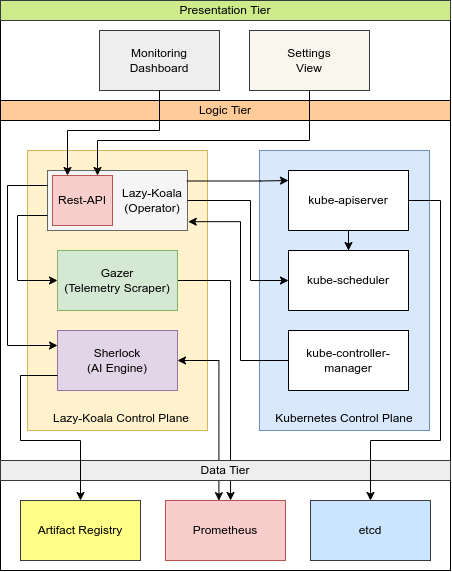
\includegraphics[width=14cm]{assets/system-design/tier-architecture.png}
    \caption{Tiered architecture (self-composed))}
    \label{fig:tier-architecture}
\end{figure}

\subsection{Presentation Tier}

The presentation tier will be entirely running in the client's computer while depending on the logic tier for data.

\begin{itemize}
    \item \textbf{Monitoring Dashboard} - This view is responsible for helping the user to understand the service topology and visually identify issues in the system.
    \item \textbf{Settings View} - On the settings page users can choose which services are needed to be monitored along with their DNS address.
\end{itemize}

\subsection{Logic Tier}

The logic tier will contain three custom microservices that depend on Kubernetes's core modules to operate.

\begin{itemize}
    \item \textbf{\ac{lazy-koala-operator}} - The \ac{lazy-koala-operator} is the main bridge between Kubernetes APIs and this system. It also contains a proxy server that securely redirects incoming client requests to kube-apiserver.
    \item \textbf{\ac{gazer}} - An instance of \ac{gazer} will be running on every node in the Kubernetes cluster which passively extracts telemetry and sends them over to the Prometheus server for later processing.
    \item \textbf{\ac{sherlock}} - AI engine periodically query Prometheus to get the current status of all the monitored service. Then it calculates an anomaly score for each service and pushes it to Prometheus so it can be sent back to the presentation layer
    \item \textbf{kube-apiserver} - This is an API provided by Kubernetes that help to read and update the cluster status programmatically.
    \item \textbf{kube-scheduler} - kube-scheduler is responsible for smartly provision requested resources in available spaces.
    \item \textbf{kube-controller-manager} - This service send updates to all the operators running on the cluster whenever there is a change to a resource that was owned by the specific operator.
\end{itemize}

\subsection{Data Tier}

\begin{itemize}
    \item \textbf{Artifact registry} - All the pre-trained models and built containers will be saved here for easy access.
    \item \textbf{Prometheus} - Prometheus is a time-series database that is highly optimized for storing service telemetry.
    \item \textbf{etcd} - etcd is an in-memory database that will be responsible for holding the resources specifications and \ac{gazer} config.
\end{itemize}
\section{System Design}

\subsection{Design Paradigm}

When building a software application there are 2 main design paradigms to choose from to organize the code structure. Object-Oriented Analysis and Design (OOAD) which is very popular among programming languages such as Java and C\# is a way of mimicking the behavior of real-world objects and how they interact real-world. However, this project has a lot of components that are loosely coupled and implemented in many different languages and frameworks Structured Systems Analysis and Design (SSADM) was chosen as the design paradigm.

\subsection{Data-flow diagram}

The Data-flow diagram explains the flow of request data within the system and how each process in the system interacts with each other at a high level.

\begin{figure}[H]
    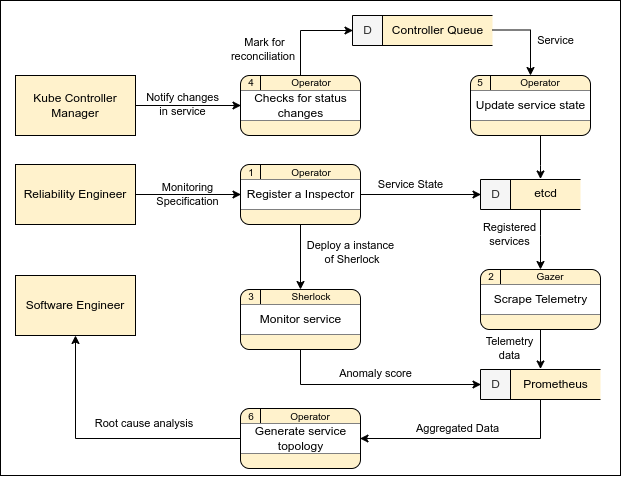
\includegraphics[width=15cm]{assets/system-design/data-flow-level-1.png}
    \caption{Data-flow diagram - level 1 (self-composed)}
    % \label{fig:data-flow}
\end{figure}

\begin{figure}[H]
    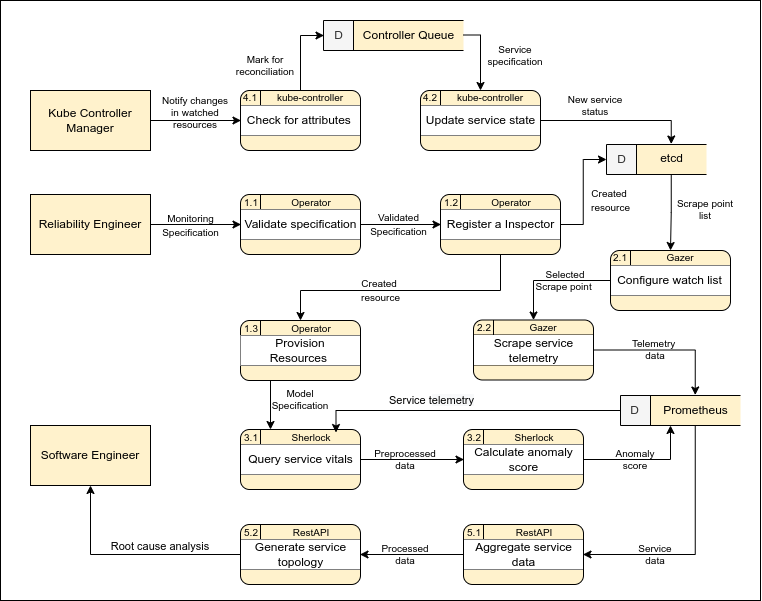
\includegraphics[width=15cm]{assets/system-design/data-flow-level-2.png}
    \caption{Data-flow diagram - level 2 (self-composed)}
    % \label{fig:data-flow}
\end{figure}


\subsection{Sequence Diagram}

Sequences diagrams are meant to showcase the flow of instructions within sub-components of the system. Digrams below explains how the system reacts when two of the main core functionality are invoked.

\begin{figure}[H]
    \centering
    \begin{subfigure}[b]{0.70\textwidth}
        \centering
        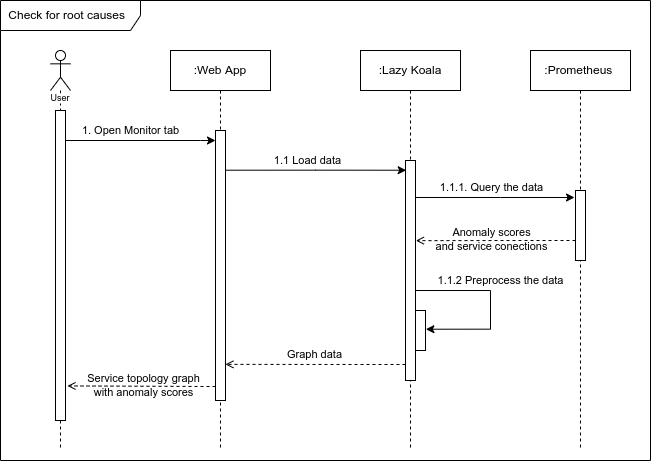
\includegraphics[width=\textwidth]{assets/system-design/sequence-diagram-1.png}
        \caption{Check for root cause}
    \end{subfigure}
    \hfill
    \begin{subfigure}[b]{0.70\textwidth}
        \centering
        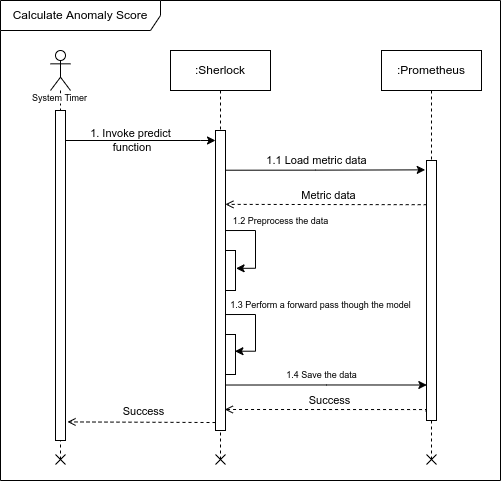
\includegraphics[width=\textwidth]{assets/system-design/sequence-diagram-2.png}
        \caption{Calculate anomaly score}
    \end{subfigure}
    \hfill
       \caption{Sequence diagrams (self-composed)}
\end{figure}

\subsection{UI Design}

Since this project was developed as a Kubernetes native application most of the functionality work as a daemon process in the background. However, there are two use cases where having a visual user interface greatly increases the usability of this project. UI mockups attached below showcase two of those use-cases. Figure \ref{fig:ui-home} displays how developers will be able to inspect the topology of the system and find issues in a realtime while, Figure \ref{fig:ui-settings} showcase the settings page which is used to tag interested services in the system which needs to be monitored.

\begin{figure}[H]
    \centering
    \begin{subfigure}[b]{0.75\textwidth}
        \centering
        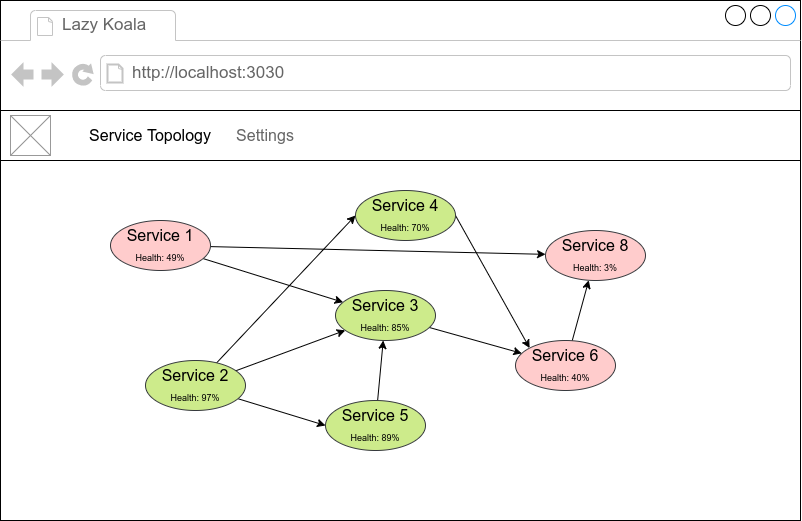
\includegraphics[width=\textwidth]{assets/system-design/ui-home.png}
        \caption{Inspector View}
        \label{fig:ui-home}
    \end{subfigure}
    \hfill
    \begin{subfigure}[b]{0.75\textwidth}
        \centering
        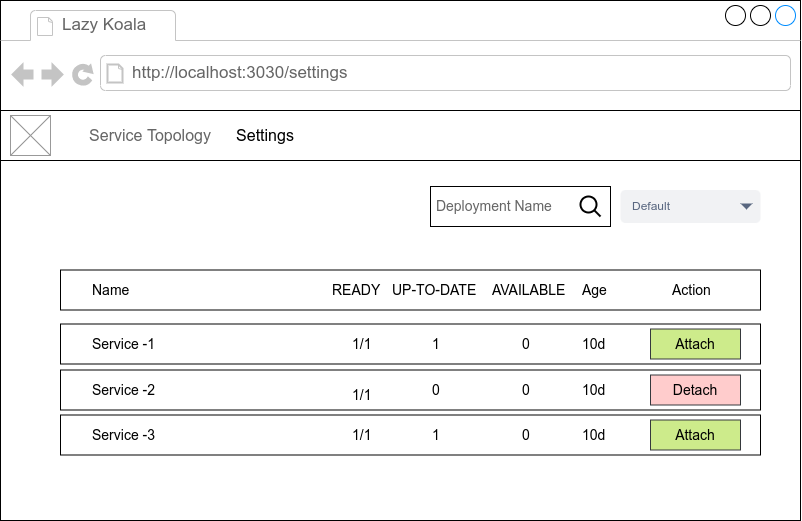
\includegraphics[width=\textwidth]{assets/system-design/ui-settings.png}
        \caption{Settings View}
        \label{fig:ui-settings}
    \end{subfigure}
    \hfill
    % \label{fig:ui-mocks}
    \caption{UI mockups (self-composed)}
\end{figure}
\section{Chapter Summary}

This chapter forced the testing process of the proposed system. During this process, the author first explained the goals and criteria of the testing process. Then the testing process and the results of the tests were presented. Finally, the chapter concluded with limitations of the testing process and what could have been done better in the future.
{\let\clearpage\relax \chapter{Initial System Design}}

\section{Chapter Overview}

% This document was made to provide the necessary context about one of the main pain points that arises when it comes to maintaining distributed systems and a course of actions that could be taken to reduce them. To do that author will first give a brief overview of the target domain and existing steps that have already been taken, then the author talks about shortcomings and improvements that can be made to them. Finally, the document will be concluded with how the author will approach the problem and try to solve it.

Cloud computing is in a steady rise for the past few years due to its scalability and ease of use. With this change, a new programming paradigm called cloud-native was born. Cloud-native applications are often developed as a set of stand-alone microservices yet could depend on each other to provide a unified experience. Even though their microservices bring a lot to the table when it comes to the flexibility it could be a nightmare to operate in production.

In this chapter the author will explain the problem domain of this research project, the specific issue this project is going to address, the motivation behind this project and its objectives and finally, concludes the chapter with novelty of the research and expected research challenges.
\section{Design Goals}
\begin{longtable}{|p{22mm}|p{131mm}|}
\hline
\textbf{Design Goal} &
    \textbf{Description} \\ \hline
    Modularity &
    Since this is designed to work in a cloud-native environment, it’s considered best practice to have all the components loosely coupled, and during the requirement engineering phase two of the industry experts, expressed their interests to integrate this project into some of their existing toolings. \\ \hline
    
    Lightweight &
    As this was designed to be a supporting system to existing distributed systems, it needs to be as lightweight as possible to justify the use of this. If the supporting system is consuming more resources than the target system it won’t be practical to use. \\ \hline
    
    No Code Change &
    It’s highly unlikely for developers to update all the services in a distributed system to match with a monitoring system. So to increase adaptability, this system should be able to work without any instrumentation from the developers’ side. \\ \hline
    
    Extensibility &
    One of the core goals of this project is to be a starting place for future researchers who are looking into root cause analysis. So having this toolkit extensible will greatly help their efforts. \\ \hline
    
    Scalability &
    Since the main target audience of this product is large enterprises with huge systems, this system should be able to scale up their level in order to be relevant. \\ \hline

    \caption{Project design goals (self-composed)}
\end{longtable}
\section{System Architecture}

System architecture design gives a birds-eye view of how all the components in the system communicate with each other. This helps us to understand the dependencies and responsibilities of each component. Since this system is designed to run on a microservices-based environment, an n-tier design architecture was used to physically separate the components in the system to have better a reliability and scalability.

\begin{figure}[H]
    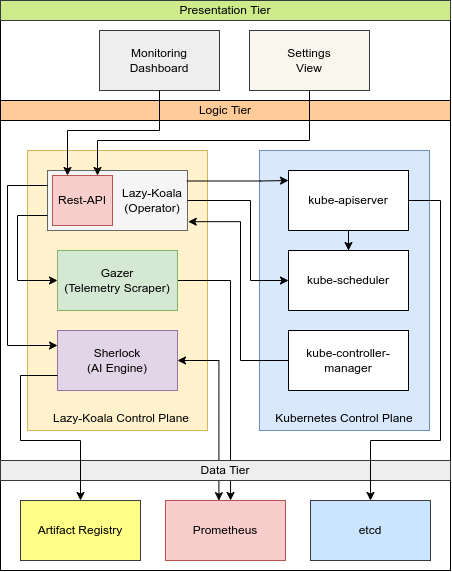
\includegraphics[width=14cm]{assets/system-design/tier-architecture.png}
    \caption{Tiered architecture (self-composed))}
    \label{fig:tier-architecture}
\end{figure}

\subsection{Presentation Tier}

The presentation tier will be entirely running in the client's computer while depending on the logic tier for data.

\begin{itemize}
    \item \textbf{Monitoring Dashboard} - This view is responsible for helping the user to understand the service topology and visually identify issues in the system.
    \item \textbf{Settings View} - On the settings page users can choose which services are needed to be monitored along with their DNS address.
\end{itemize}

\subsection{Logic Tier}

The logic tier will contain three custom microservices that depend on Kubernetes's core modules to operate.

\begin{itemize}
    \item \textbf{\ac{lazy-koala-operator}} - The \ac{lazy-koala-operator} is the main bridge between Kubernetes APIs and this system. It also contains a proxy server that securely redirects incoming client requests to kube-apiserver.
    \item \textbf{\ac{gazer}} - An instance of \ac{gazer} will be running on every node in the Kubernetes cluster which passively extracts telemetry and sends them over to the Prometheus server for later processing.
    \item \textbf{\ac{sherlock}} - AI engine periodically query Prometheus to get the current status of all the monitored service. Then it calculates an anomaly score for each service and pushes it to Prometheus so it can be sent back to the presentation layer
    \item \textbf{kube-apiserver} - This is an API provided by Kubernetes that help to read and update the cluster status programmatically.
    \item \textbf{kube-scheduler} - kube-scheduler is responsible for smartly provision requested resources in available spaces.
    \item \textbf{kube-controller-manager} - This service send updates to all the operators running on the cluster whenever there is a change to a resource that was owned by the specific operator.
\end{itemize}

\subsection{Data Tier}

\begin{itemize}
    \item \textbf{Artifact registry} - All the pre-trained models and built containers will be saved here for easy access.
    \item \textbf{Prometheus} - Prometheus is a time-series database that is highly optimized for storing service telemetry.
    \item \textbf{etcd} - etcd is an in-memory database that will be responsible for holding the resources specifications and \ac{gazer} config.
\end{itemize}
\section{System Design}

\subsection{Design Paradigm}

When building a software application there are 2 main design paradigms to choose from to organize the code structure. Object-Oriented Analysis and Design (OOAD) which is very popular among programming languages such as Java and C\# is a way of mimicking the behavior of real-world objects and how they interact real-world. However, this project has a lot of components that are loosely coupled and implemented in many different languages and frameworks Structured Systems Analysis and Design (SSADM) was chosen as the design paradigm.

\subsection{Data-flow diagram}

The Data-flow diagram explains the flow of request data within the system and how each process in the system interacts with each other at a high level.

\begin{figure}[H]
    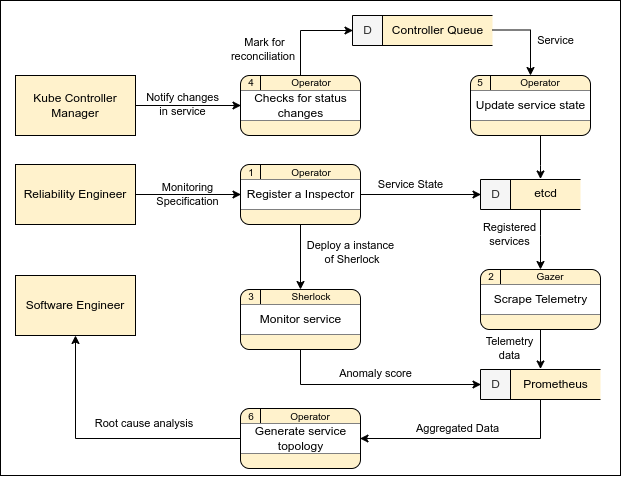
\includegraphics[width=15cm]{assets/system-design/data-flow-level-1.png}
    \caption{Data-flow diagram - level 1 (self-composed)}
    % \label{fig:data-flow}
\end{figure}

\begin{figure}[H]
    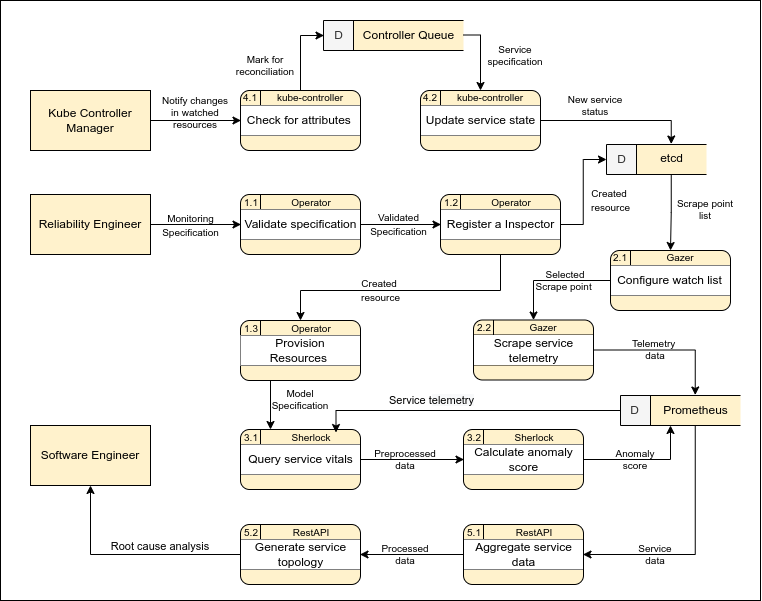
\includegraphics[width=15cm]{assets/system-design/data-flow-level-2.png}
    \caption{Data-flow diagram - level 2 (self-composed)}
    % \label{fig:data-flow}
\end{figure}


\subsection{Sequence Diagram}

Sequences diagrams are meant to showcase the flow of instructions within sub-components of the system. Digrams below explains how the system reacts when two of the main core functionality are invoked.

\begin{figure}[H]
    \centering
    \begin{subfigure}[b]{0.70\textwidth}
        \centering
        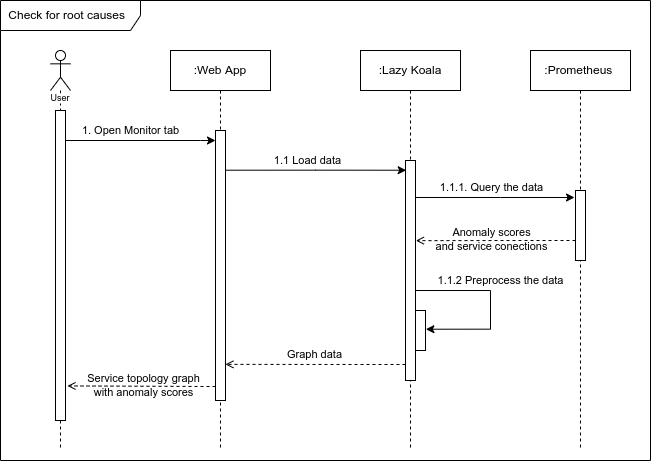
\includegraphics[width=\textwidth]{assets/system-design/sequence-diagram-1.png}
        \caption{Check for root cause}
    \end{subfigure}
    \hfill
    \begin{subfigure}[b]{0.70\textwidth}
        \centering
        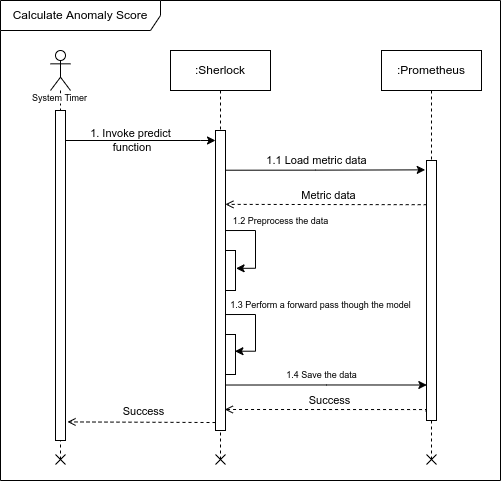
\includegraphics[width=\textwidth]{assets/system-design/sequence-diagram-2.png}
        \caption{Calculate anomaly score}
    \end{subfigure}
    \hfill
       \caption{Sequence diagrams (self-composed)}
\end{figure}

\subsection{UI Design}

Since this project was developed as a Kubernetes native application most of the functionality work as a daemon process in the background. However, there are two use cases where having a visual user interface greatly increases the usability of this project. UI mockups attached below showcase two of those use-cases. Figure \ref{fig:ui-home} displays how developers will be able to inspect the topology of the system and find issues in a realtime while, Figure \ref{fig:ui-settings} showcase the settings page which is used to tag interested services in the system which needs to be monitored.

\begin{figure}[H]
    \centering
    \begin{subfigure}[b]{0.75\textwidth}
        \centering
        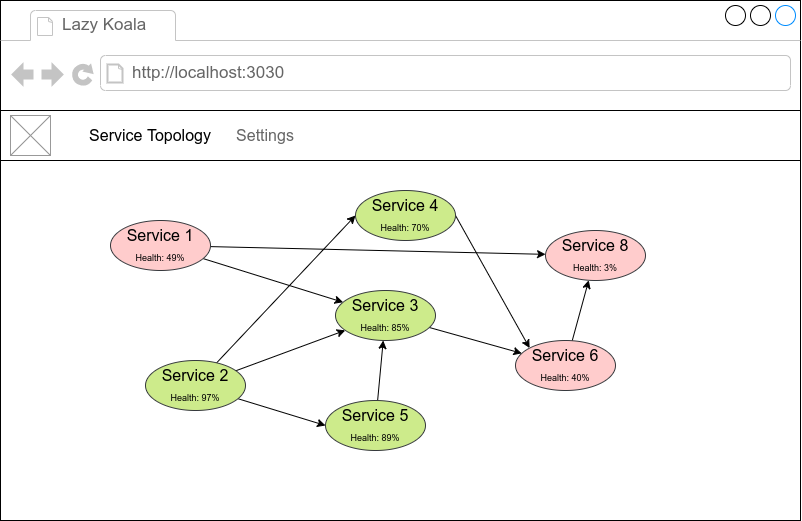
\includegraphics[width=\textwidth]{assets/system-design/ui-home.png}
        \caption{Inspector View}
        \label{fig:ui-home}
    \end{subfigure}
    \hfill
    \begin{subfigure}[b]{0.75\textwidth}
        \centering
        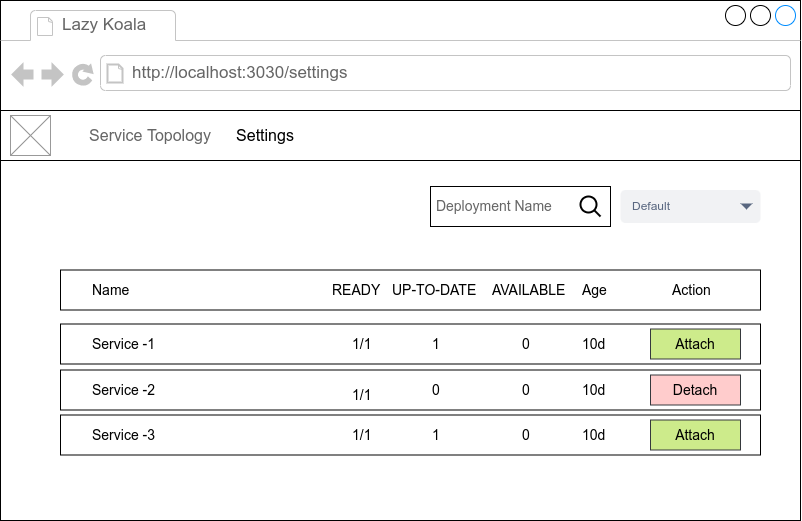
\includegraphics[width=\textwidth]{assets/system-design/ui-settings.png}
        \caption{Settings View}
        \label{fig:ui-settings}
    \end{subfigure}
    \hfill
    % \label{fig:ui-mocks}
    \caption{UI mockups (self-composed)}
\end{figure}
\section{Chapter Summary}

This chapter forced the testing process of the proposed system. During this process, the author first explained the goals and criteria of the testing process. Then the testing process and the results of the tests were presented. Finally, the chapter concluded with limitations of the testing process and what could have been done better in the future.
{\let\clearpage\relax \chapter{Initial System Design}}

\section{Chapter Overview}

% This document was made to provide the necessary context about one of the main pain points that arises when it comes to maintaining distributed systems and a course of actions that could be taken to reduce them. To do that author will first give a brief overview of the target domain and existing steps that have already been taken, then the author talks about shortcomings and improvements that can be made to them. Finally, the document will be concluded with how the author will approach the problem and try to solve it.

Cloud computing is in a steady rise for the past few years due to its scalability and ease of use. With this change, a new programming paradigm called cloud-native was born. Cloud-native applications are often developed as a set of stand-alone microservices yet could depend on each other to provide a unified experience. Even though their microservices bring a lot to the table when it comes to the flexibility it could be a nightmare to operate in production.

In this chapter the author will explain the problem domain of this research project, the specific issue this project is going to address, the motivation behind this project and its objectives and finally, concludes the chapter with novelty of the research and expected research challenges.
\section{Design Goals}
\begin{longtable}{|p{22mm}|p{131mm}|}
\hline
\textbf{Design Goal} &
    \textbf{Description} \\ \hline
    Modularity &
    Since this is designed to work in a cloud-native environment, it’s considered best practice to have all the components loosely coupled, and during the requirement engineering phase two of the industry experts, expressed their interests to integrate this project into some of their existing toolings. \\ \hline
    
    Lightweight &
    As this was designed to be a supporting system to existing distributed systems, it needs to be as lightweight as possible to justify the use of this. If the supporting system is consuming more resources than the target system it won’t be practical to use. \\ \hline
    
    No Code Change &
    It’s highly unlikely for developers to update all the services in a distributed system to match with a monitoring system. So to increase adaptability, this system should be able to work without any instrumentation from the developers’ side. \\ \hline
    
    Extensibility &
    One of the core goals of this project is to be a starting place for future researchers who are looking into root cause analysis. So having this toolkit extensible will greatly help their efforts. \\ \hline
    
    Scalability &
    Since the main target audience of this product is large enterprises with huge systems, this system should be able to scale up their level in order to be relevant. \\ \hline

    \caption{Project design goals (self-composed)}
\end{longtable}
\section{System Architecture}

System architecture design gives a birds-eye view of how all the components in the system communicate with each other. This helps us to understand the dependencies and responsibilities of each component. Since this system is designed to run on a microservices-based environment, an n-tier design architecture was used to physically separate the components in the system to have better a reliability and scalability.

\begin{figure}[H]
    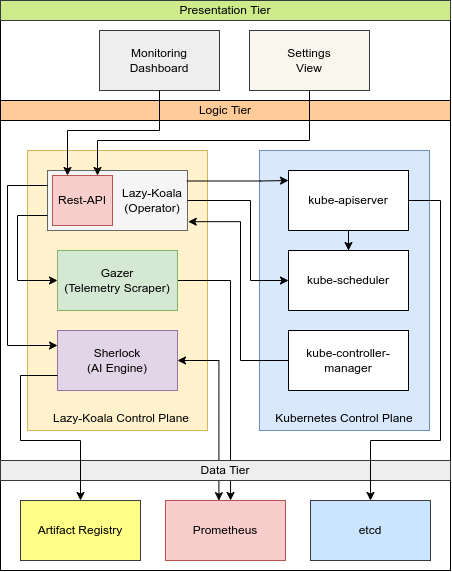
\includegraphics[width=14cm]{assets/system-design/tier-architecture.png}
    \caption{Tiered architecture (self-composed))}
    \label{fig:tier-architecture}
\end{figure}

\subsection{Presentation Tier}

The presentation tier will be entirely running in the client's computer while depending on the logic tier for data.

\begin{itemize}
    \item \textbf{Monitoring Dashboard} - This view is responsible for helping the user to understand the service topology and visually identify issues in the system.
    \item \textbf{Settings View} - On the settings page users can choose which services are needed to be monitored along with their DNS address.
\end{itemize}

\subsection{Logic Tier}

The logic tier will contain three custom microservices that depend on Kubernetes's core modules to operate.

\begin{itemize}
    \item \textbf{\ac{lazy-koala-operator}} - The \ac{lazy-koala-operator} is the main bridge between Kubernetes APIs and this system. It also contains a proxy server that securely redirects incoming client requests to kube-apiserver.
    \item \textbf{\ac{gazer}} - An instance of \ac{gazer} will be running on every node in the Kubernetes cluster which passively extracts telemetry and sends them over to the Prometheus server for later processing.
    \item \textbf{\ac{sherlock}} - AI engine periodically query Prometheus to get the current status of all the monitored service. Then it calculates an anomaly score for each service and pushes it to Prometheus so it can be sent back to the presentation layer
    \item \textbf{kube-apiserver} - This is an API provided by Kubernetes that help to read and update the cluster status programmatically.
    \item \textbf{kube-scheduler} - kube-scheduler is responsible for smartly provision requested resources in available spaces.
    \item \textbf{kube-controller-manager} - This service send updates to all the operators running on the cluster whenever there is a change to a resource that was owned by the specific operator.
\end{itemize}

\subsection{Data Tier}

\begin{itemize}
    \item \textbf{Artifact registry} - All the pre-trained models and built containers will be saved here for easy access.
    \item \textbf{Prometheus} - Prometheus is a time-series database that is highly optimized for storing service telemetry.
    \item \textbf{etcd} - etcd is an in-memory database that will be responsible for holding the resources specifications and \ac{gazer} config.
\end{itemize}
\section{System Design}

\subsection{Design Paradigm}

When building a software application there are 2 main design paradigms to choose from to organize the code structure. Object-Oriented Analysis and Design (OOAD) which is very popular among programming languages such as Java and C\# is a way of mimicking the behavior of real-world objects and how they interact real-world. However, this project has a lot of components that are loosely coupled and implemented in many different languages and frameworks Structured Systems Analysis and Design (SSADM) was chosen as the design paradigm.

\subsection{Data-flow diagram}

The Data-flow diagram explains the flow of request data within the system and how each process in the system interacts with each other at a high level.

\begin{figure}[H]
    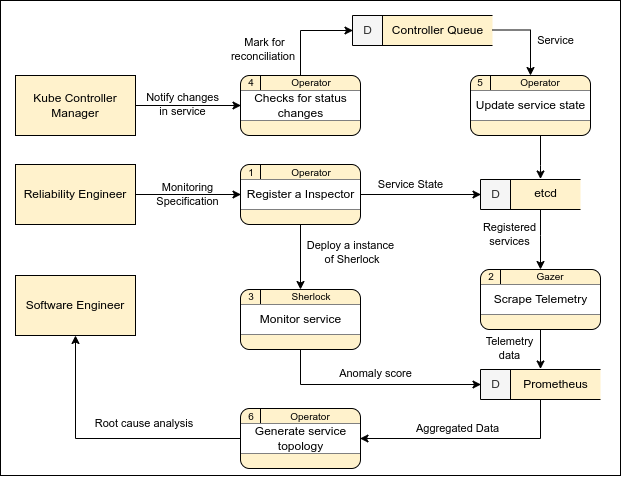
\includegraphics[width=15cm]{assets/system-design/data-flow-level-1.png}
    \caption{Data-flow diagram - level 1 (self-composed)}
    % \label{fig:data-flow}
\end{figure}

\begin{figure}[H]
    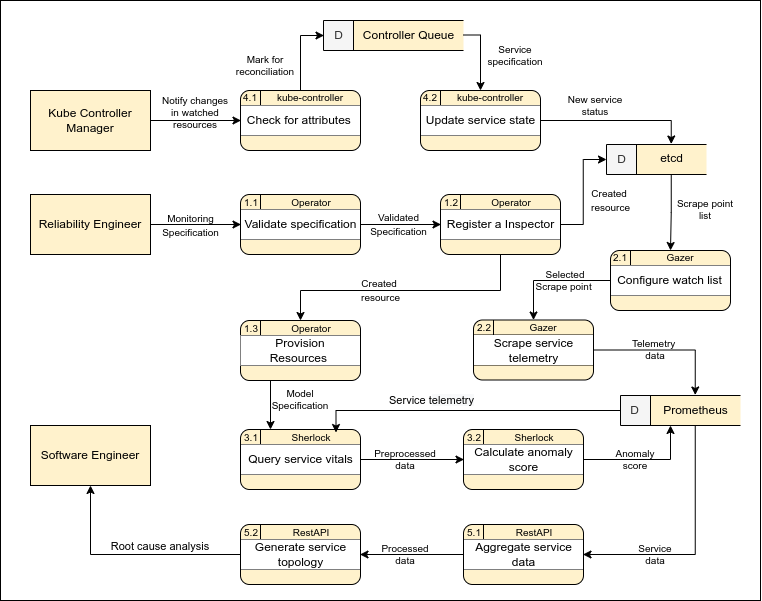
\includegraphics[width=15cm]{assets/system-design/data-flow-level-2.png}
    \caption{Data-flow diagram - level 2 (self-composed)}
    % \label{fig:data-flow}
\end{figure}


\subsection{Sequence Diagram}

Sequences diagrams are meant to showcase the flow of instructions within sub-components of the system. Digrams below explains how the system reacts when two of the main core functionality are invoked.

\begin{figure}[H]
    \centering
    \begin{subfigure}[b]{0.70\textwidth}
        \centering
        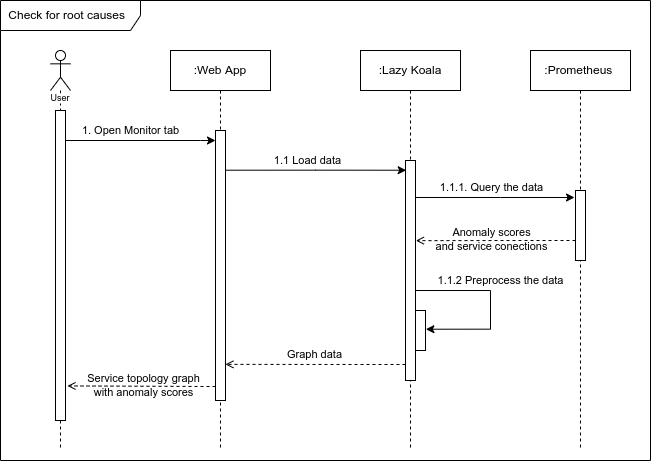
\includegraphics[width=\textwidth]{assets/system-design/sequence-diagram-1.png}
        \caption{Check for root cause}
    \end{subfigure}
    \hfill
    \begin{subfigure}[b]{0.70\textwidth}
        \centering
        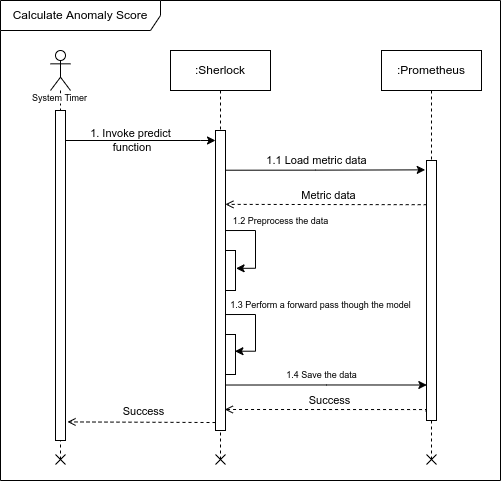
\includegraphics[width=\textwidth]{assets/system-design/sequence-diagram-2.png}
        \caption{Calculate anomaly score}
    \end{subfigure}
    \hfill
       \caption{Sequence diagrams (self-composed)}
\end{figure}

\subsection{UI Design}

Since this project was developed as a Kubernetes native application most of the functionality work as a daemon process in the background. However, there are two use cases where having a visual user interface greatly increases the usability of this project. UI mockups attached below showcase two of those use-cases. Figure \ref{fig:ui-home} displays how developers will be able to inspect the topology of the system and find issues in a realtime while, Figure \ref{fig:ui-settings} showcase the settings page which is used to tag interested services in the system which needs to be monitored.

\begin{figure}[H]
    \centering
    \begin{subfigure}[b]{0.75\textwidth}
        \centering
        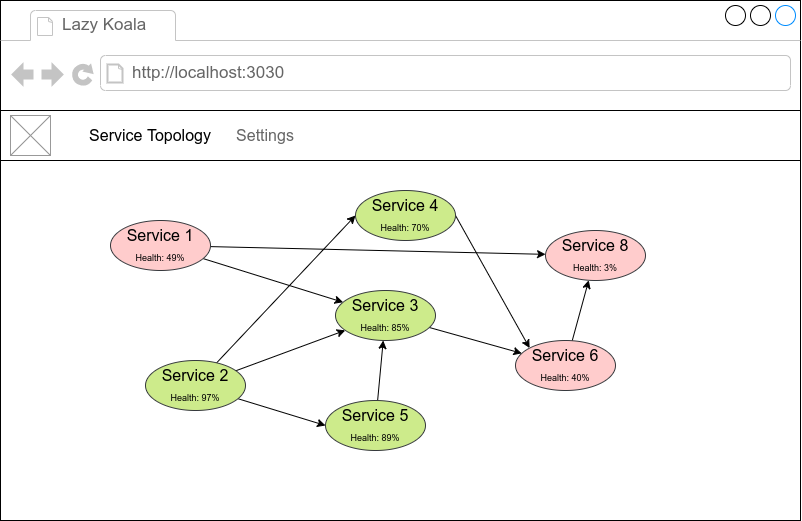
\includegraphics[width=\textwidth]{assets/system-design/ui-home.png}
        \caption{Inspector View}
        \label{fig:ui-home}
    \end{subfigure}
    \hfill
    \begin{subfigure}[b]{0.75\textwidth}
        \centering
        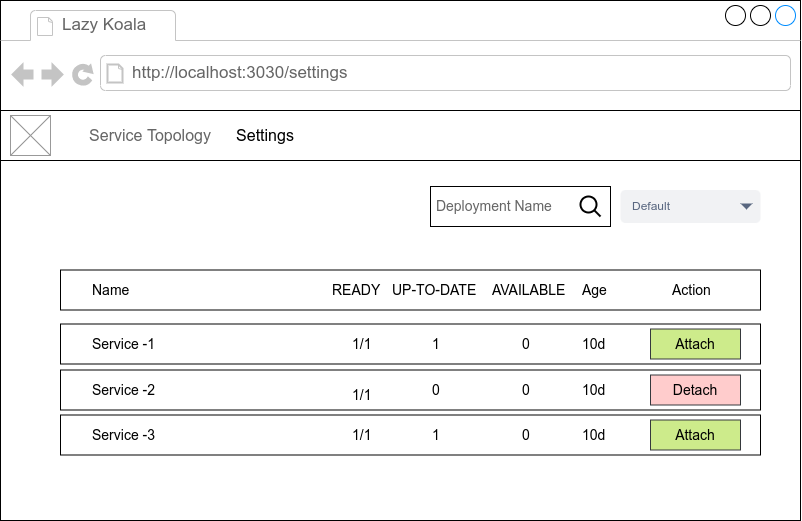
\includegraphics[width=\textwidth]{assets/system-design/ui-settings.png}
        \caption{Settings View}
        \label{fig:ui-settings}
    \end{subfigure}
    \hfill
    % \label{fig:ui-mocks}
    \caption{UI mockups (self-composed)}
\end{figure}
\section{Chapter Summary}

This chapter forced the testing process of the proposed system. During this process, the author first explained the goals and criteria of the testing process. Then the testing process and the results of the tests were presented. Finally, the chapter concluded with limitations of the testing process and what could have been done better in the future.
{\let\clearpage\relax \chapter{Initial System Design}}

\section{Chapter Overview}

% This document was made to provide the necessary context about one of the main pain points that arises when it comes to maintaining distributed systems and a course of actions that could be taken to reduce them. To do that author will first give a brief overview of the target domain and existing steps that have already been taken, then the author talks about shortcomings and improvements that can be made to them. Finally, the document will be concluded with how the author will approach the problem and try to solve it.

Cloud computing is in a steady rise for the past few years due to its scalability and ease of use. With this change, a new programming paradigm called cloud-native was born. Cloud-native applications are often developed as a set of stand-alone microservices yet could depend on each other to provide a unified experience. Even though their microservices bring a lot to the table when it comes to the flexibility it could be a nightmare to operate in production.

In this chapter the author will explain the problem domain of this research project, the specific issue this project is going to address, the motivation behind this project and its objectives and finally, concludes the chapter with novelty of the research and expected research challenges.
\section{Design Goals}
\begin{longtable}{|p{22mm}|p{131mm}|}
\hline
\textbf{Design Goal} &
    \textbf{Description} \\ \hline
    Modularity &
    Since this is designed to work in a cloud-native environment, it’s considered best practice to have all the components loosely coupled, and during the requirement engineering phase two of the industry experts, expressed their interests to integrate this project into some of their existing toolings. \\ \hline
    
    Lightweight &
    As this was designed to be a supporting system to existing distributed systems, it needs to be as lightweight as possible to justify the use of this. If the supporting system is consuming more resources than the target system it won’t be practical to use. \\ \hline
    
    No Code Change &
    It’s highly unlikely for developers to update all the services in a distributed system to match with a monitoring system. So to increase adaptability, this system should be able to work without any instrumentation from the developers’ side. \\ \hline
    
    Extensibility &
    One of the core goals of this project is to be a starting place for future researchers who are looking into root cause analysis. So having this toolkit extensible will greatly help their efforts. \\ \hline
    
    Scalability &
    Since the main target audience of this product is large enterprises with huge systems, this system should be able to scale up their level in order to be relevant. \\ \hline

    \caption{Project design goals (self-composed)}
\end{longtable}
\section{System Architecture}

System architecture design gives a birds-eye view of how all the components in the system communicate with each other. This helps us to understand the dependencies and responsibilities of each component. Since this system is designed to run on a microservices-based environment, an n-tier design architecture was used to physically separate the components in the system to have better a reliability and scalability.

\begin{figure}[H]
    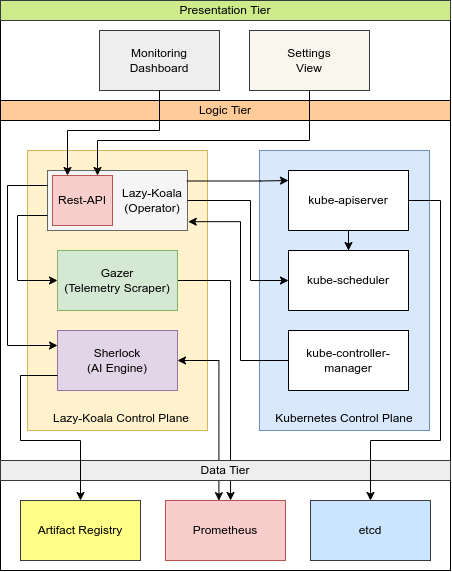
\includegraphics[width=14cm]{assets/system-design/tier-architecture.png}
    \caption{Tiered architecture (self-composed))}
    \label{fig:tier-architecture}
\end{figure}

\subsection{Presentation Tier}

The presentation tier will be entirely running in the client's computer while depending on the logic tier for data.

\begin{itemize}
    \item \textbf{Monitoring Dashboard} - This view is responsible for helping the user to understand the service topology and visually identify issues in the system.
    \item \textbf{Settings View} - On the settings page users can choose which services are needed to be monitored along with their DNS address.
\end{itemize}

\subsection{Logic Tier}

The logic tier will contain three custom microservices that depend on Kubernetes's core modules to operate.

\begin{itemize}
    \item \textbf{\ac{lazy-koala-operator}} - The \ac{lazy-koala-operator} is the main bridge between Kubernetes APIs and this system. It also contains a proxy server that securely redirects incoming client requests to kube-apiserver.
    \item \textbf{\ac{gazer}} - An instance of \ac{gazer} will be running on every node in the Kubernetes cluster which passively extracts telemetry and sends them over to the Prometheus server for later processing.
    \item \textbf{\ac{sherlock}} - AI engine periodically query Prometheus to get the current status of all the monitored service. Then it calculates an anomaly score for each service and pushes it to Prometheus so it can be sent back to the presentation layer
    \item \textbf{kube-apiserver} - This is an API provided by Kubernetes that help to read and update the cluster status programmatically.
    \item \textbf{kube-scheduler} - kube-scheduler is responsible for smartly provision requested resources in available spaces.
    \item \textbf{kube-controller-manager} - This service send updates to all the operators running on the cluster whenever there is a change to a resource that was owned by the specific operator.
\end{itemize}

\subsection{Data Tier}

\begin{itemize}
    \item \textbf{Artifact registry} - All the pre-trained models and built containers will be saved here for easy access.
    \item \textbf{Prometheus} - Prometheus is a time-series database that is highly optimized for storing service telemetry.
    \item \textbf{etcd} - etcd is an in-memory database that will be responsible for holding the resources specifications and \ac{gazer} config.
\end{itemize}
\section{System Design}

\subsection{Design Paradigm}

When building a software application there are 2 main design paradigms to choose from to organize the code structure. Object-Oriented Analysis and Design (OOAD) which is very popular among programming languages such as Java and C\# is a way of mimicking the behavior of real-world objects and how they interact real-world. However, this project has a lot of components that are loosely coupled and implemented in many different languages and frameworks Structured Systems Analysis and Design (SSADM) was chosen as the design paradigm.

\subsection{Data-flow diagram}

The Data-flow diagram explains the flow of request data within the system and how each process in the system interacts with each other at a high level.

\begin{figure}[H]
    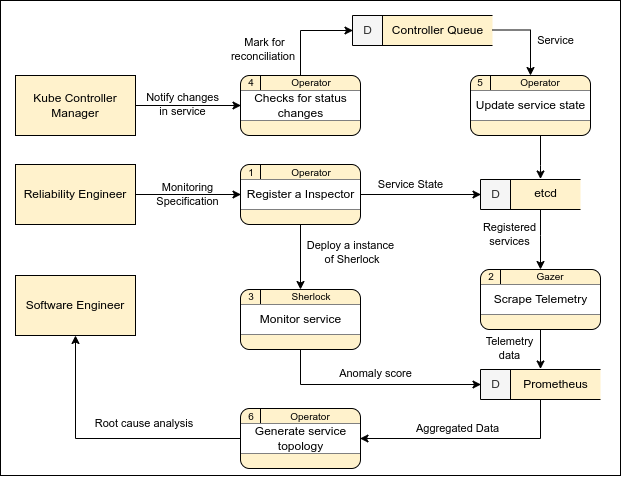
\includegraphics[width=15cm]{assets/system-design/data-flow-level-1.png}
    \caption{Data-flow diagram - level 1 (self-composed)}
    % \label{fig:data-flow}
\end{figure}

\begin{figure}[H]
    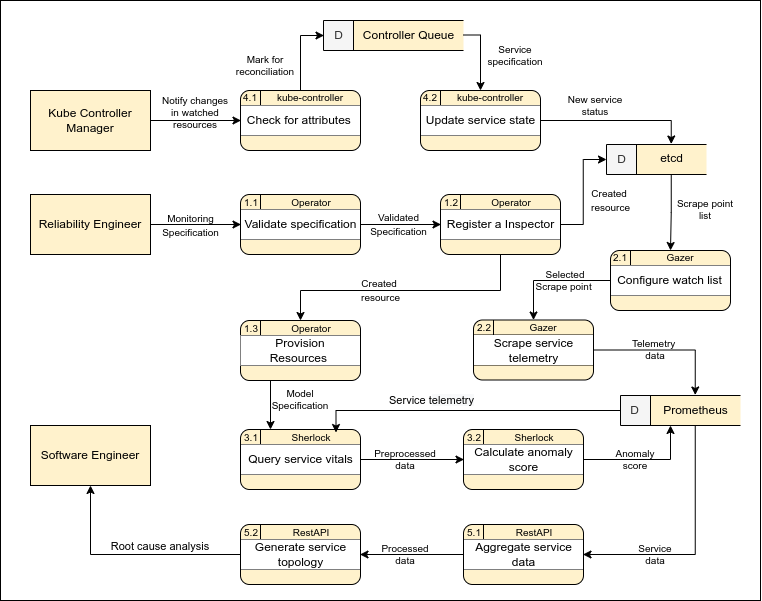
\includegraphics[width=15cm]{assets/system-design/data-flow-level-2.png}
    \caption{Data-flow diagram - level 2 (self-composed)}
    % \label{fig:data-flow}
\end{figure}


\subsection{Sequence Diagram}

Sequences diagrams are meant to showcase the flow of instructions within sub-components of the system. Digrams below explains how the system reacts when two of the main core functionality are invoked.

\begin{figure}[H]
    \centering
    \begin{subfigure}[b]{0.70\textwidth}
        \centering
        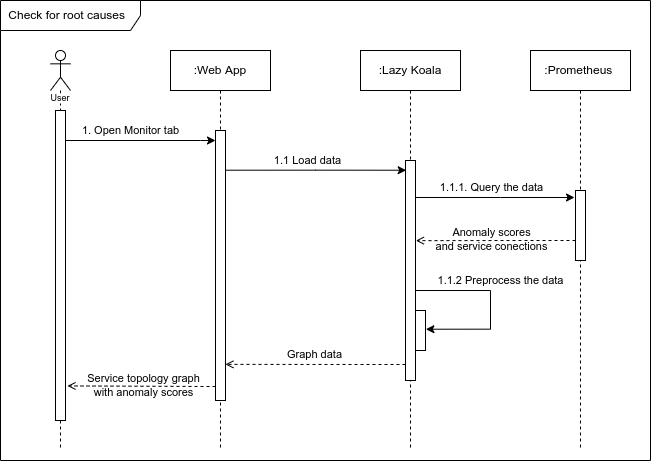
\includegraphics[width=\textwidth]{assets/system-design/sequence-diagram-1.png}
        \caption{Check for root cause}
    \end{subfigure}
    \hfill
    \begin{subfigure}[b]{0.70\textwidth}
        \centering
        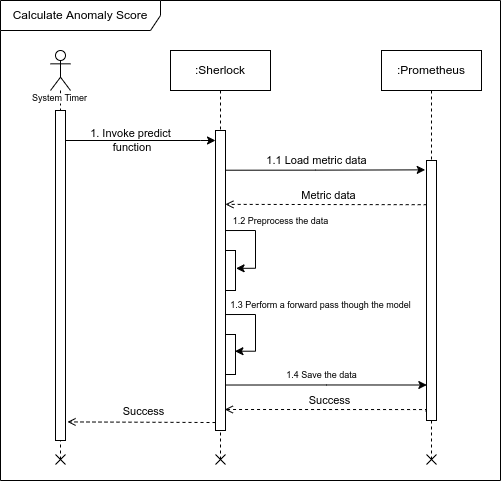
\includegraphics[width=\textwidth]{assets/system-design/sequence-diagram-2.png}
        \caption{Calculate anomaly score}
    \end{subfigure}
    \hfill
       \caption{Sequence diagrams (self-composed)}
\end{figure}

\subsection{UI Design}

Since this project was developed as a Kubernetes native application most of the functionality work as a daemon process in the background. However, there are two use cases where having a visual user interface greatly increases the usability of this project. UI mockups attached below showcase two of those use-cases. Figure \ref{fig:ui-home} displays how developers will be able to inspect the topology of the system and find issues in a realtime while, Figure \ref{fig:ui-settings} showcase the settings page which is used to tag interested services in the system which needs to be monitored.

\begin{figure}[H]
    \centering
    \begin{subfigure}[b]{0.75\textwidth}
        \centering
        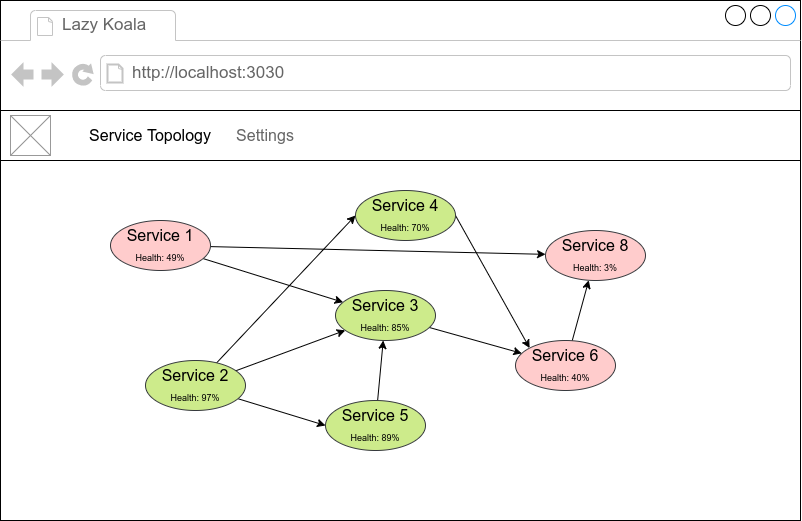
\includegraphics[width=\textwidth]{assets/system-design/ui-home.png}
        \caption{Inspector View}
        \label{fig:ui-home}
    \end{subfigure}
    \hfill
    \begin{subfigure}[b]{0.75\textwidth}
        \centering
        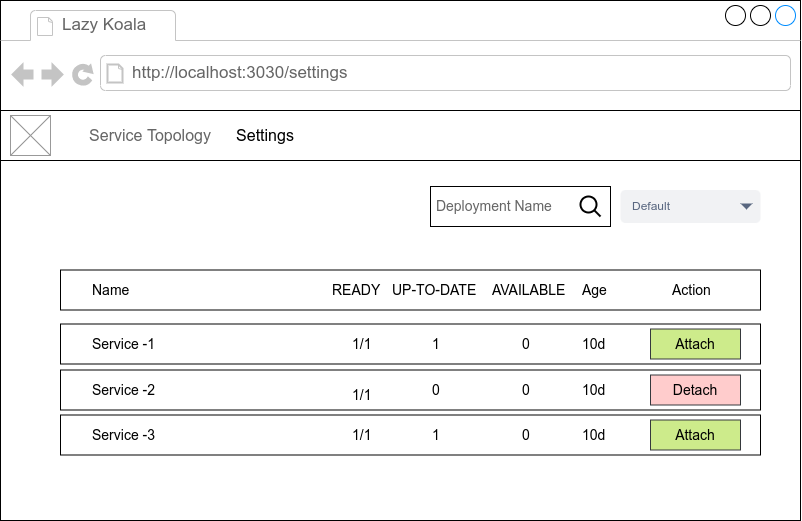
\includegraphics[width=\textwidth]{assets/system-design/ui-settings.png}
        \caption{Settings View}
        \label{fig:ui-settings}
    \end{subfigure}
    \hfill
    % \label{fig:ui-mocks}
    \caption{UI mockups (self-composed)}
\end{figure}
\section{Chapter Summary}

This chapter forced the testing process of the proposed system. During this process, the author first explained the goals and criteria of the testing process. Then the testing process and the results of the tests were presented. Finally, the chapter concluded with limitations of the testing process and what could have been done better in the future.

\cleardoublepage
\phantomsection
\renewcommand{\bibname}{References}
\pagenumbering{Roman}
% \setcounter{page}{5}
\addcontentsline{toc}{chapter}{References}
\bibliography{references.bib}

{\let\clearpage\relax \chapter{Initial System Design}}

\section{Chapter Overview}

% This document was made to provide the necessary context about one of the main pain points that arises when it comes to maintaining distributed systems and a course of actions that could be taken to reduce them. To do that author will first give a brief overview of the target domain and existing steps that have already been taken, then the author talks about shortcomings and improvements that can be made to them. Finally, the document will be concluded with how the author will approach the problem and try to solve it.

Cloud computing is in a steady rise for the past few years due to its scalability and ease of use. With this change, a new programming paradigm called cloud-native was born. Cloud-native applications are often developed as a set of stand-alone microservices yet could depend on each other to provide a unified experience. Even though their microservices bring a lot to the table when it comes to the flexibility it could be a nightmare to operate in production.

In this chapter the author will explain the problem domain of this research project, the specific issue this project is going to address, the motivation behind this project and its objectives and finally, concludes the chapter with novelty of the research and expected research challenges.
\section{Design Goals}
\begin{longtable}{|p{22mm}|p{131mm}|}
\hline
\textbf{Design Goal} &
    \textbf{Description} \\ \hline
    Modularity &
    Since this is designed to work in a cloud-native environment, it’s considered best practice to have all the components loosely coupled, and during the requirement engineering phase two of the industry experts, expressed their interests to integrate this project into some of their existing toolings. \\ \hline
    
    Lightweight &
    As this was designed to be a supporting system to existing distributed systems, it needs to be as lightweight as possible to justify the use of this. If the supporting system is consuming more resources than the target system it won’t be practical to use. \\ \hline
    
    No Code Change &
    It’s highly unlikely for developers to update all the services in a distributed system to match with a monitoring system. So to increase adaptability, this system should be able to work without any instrumentation from the developers’ side. \\ \hline
    
    Extensibility &
    One of the core goals of this project is to be a starting place for future researchers who are looking into root cause analysis. So having this toolkit extensible will greatly help their efforts. \\ \hline
    
    Scalability &
    Since the main target audience of this product is large enterprises with huge systems, this system should be able to scale up their level in order to be relevant. \\ \hline

    \caption{Project design goals (self-composed)}
\end{longtable}
\section{System Architecture}

System architecture design gives a birds-eye view of how all the components in the system communicate with each other. This helps us to understand the dependencies and responsibilities of each component. Since this system is designed to run on a microservices-based environment, an n-tier design architecture was used to physically separate the components in the system to have better a reliability and scalability.

\begin{figure}[H]
    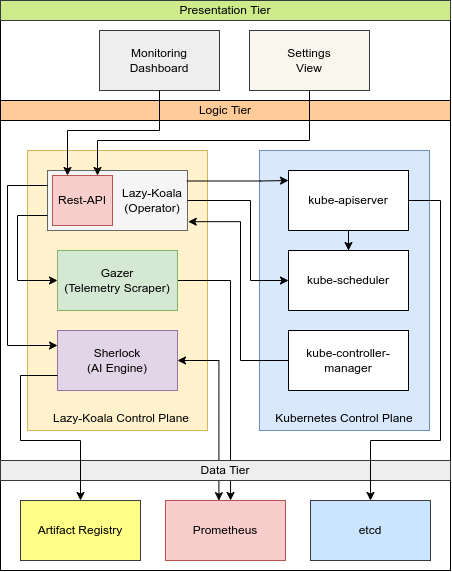
\includegraphics[width=14cm]{assets/system-design/tier-architecture.png}
    \caption{Tiered architecture (self-composed))}
    \label{fig:tier-architecture}
\end{figure}

\subsection{Presentation Tier}

The presentation tier will be entirely running in the client's computer while depending on the logic tier for data.

\begin{itemize}
    \item \textbf{Monitoring Dashboard} - This view is responsible for helping the user to understand the service topology and visually identify issues in the system.
    \item \textbf{Settings View} - On the settings page users can choose which services are needed to be monitored along with their DNS address.
\end{itemize}

\subsection{Logic Tier}

The logic tier will contain three custom microservices that depend on Kubernetes's core modules to operate.

\begin{itemize}
    \item \textbf{\ac{lazy-koala-operator}} - The \ac{lazy-koala-operator} is the main bridge between Kubernetes APIs and this system. It also contains a proxy server that securely redirects incoming client requests to kube-apiserver.
    \item \textbf{\ac{gazer}} - An instance of \ac{gazer} will be running on every node in the Kubernetes cluster which passively extracts telemetry and sends them over to the Prometheus server for later processing.
    \item \textbf{\ac{sherlock}} - AI engine periodically query Prometheus to get the current status of all the monitored service. Then it calculates an anomaly score for each service and pushes it to Prometheus so it can be sent back to the presentation layer
    \item \textbf{kube-apiserver} - This is an API provided by Kubernetes that help to read and update the cluster status programmatically.
    \item \textbf{kube-scheduler} - kube-scheduler is responsible for smartly provision requested resources in available spaces.
    \item \textbf{kube-controller-manager} - This service send updates to all the operators running on the cluster whenever there is a change to a resource that was owned by the specific operator.
\end{itemize}

\subsection{Data Tier}

\begin{itemize}
    \item \textbf{Artifact registry} - All the pre-trained models and built containers will be saved here for easy access.
    \item \textbf{Prometheus} - Prometheus is a time-series database that is highly optimized for storing service telemetry.
    \item \textbf{etcd} - etcd is an in-memory database that will be responsible for holding the resources specifications and \ac{gazer} config.
\end{itemize}
\section{System Design}

\subsection{Design Paradigm}

When building a software application there are 2 main design paradigms to choose from to organize the code structure. Object-Oriented Analysis and Design (OOAD) which is very popular among programming languages such as Java and C\# is a way of mimicking the behavior of real-world objects and how they interact real-world. However, this project has a lot of components that are loosely coupled and implemented in many different languages and frameworks Structured Systems Analysis and Design (SSADM) was chosen as the design paradigm.

\subsection{Data-flow diagram}

The Data-flow diagram explains the flow of request data within the system and how each process in the system interacts with each other at a high level.

\begin{figure}[H]
    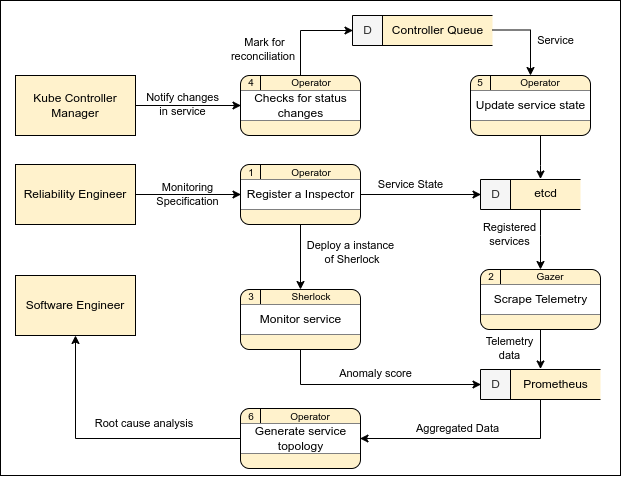
\includegraphics[width=15cm]{assets/system-design/data-flow-level-1.png}
    \caption{Data-flow diagram - level 1 (self-composed)}
    % \label{fig:data-flow}
\end{figure}

\begin{figure}[H]
    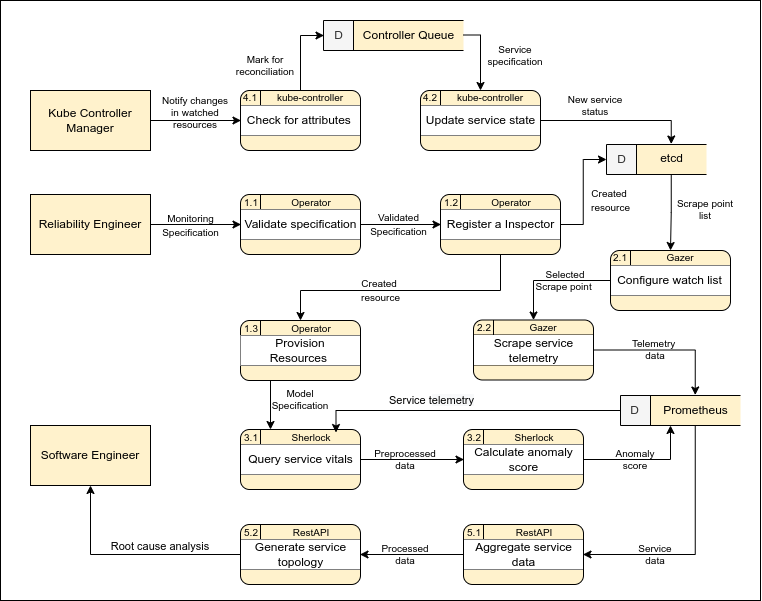
\includegraphics[width=15cm]{assets/system-design/data-flow-level-2.png}
    \caption{Data-flow diagram - level 2 (self-composed)}
    % \label{fig:data-flow}
\end{figure}


\subsection{Sequence Diagram}

Sequences diagrams are meant to showcase the flow of instructions within sub-components of the system. Digrams below explains how the system reacts when two of the main core functionality are invoked.

\begin{figure}[H]
    \centering
    \begin{subfigure}[b]{0.70\textwidth}
        \centering
        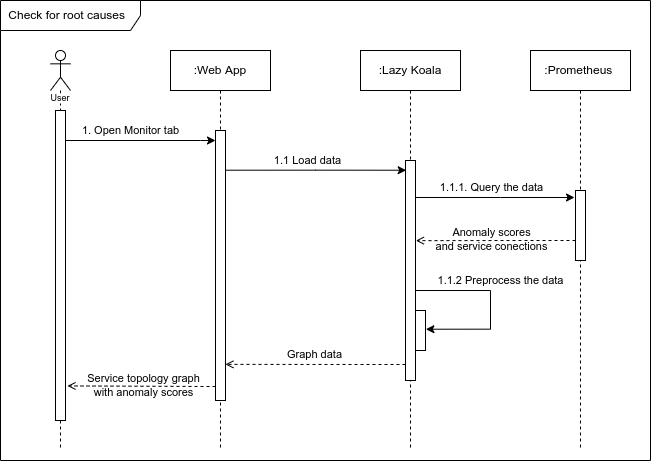
\includegraphics[width=\textwidth]{assets/system-design/sequence-diagram-1.png}
        \caption{Check for root cause}
    \end{subfigure}
    \hfill
    \begin{subfigure}[b]{0.70\textwidth}
        \centering
        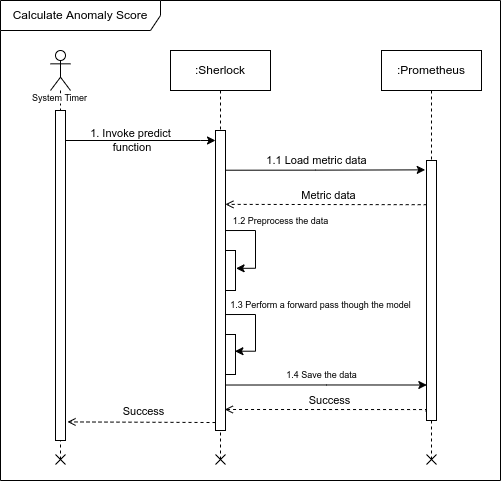
\includegraphics[width=\textwidth]{assets/system-design/sequence-diagram-2.png}
        \caption{Calculate anomaly score}
    \end{subfigure}
    \hfill
       \caption{Sequence diagrams (self-composed)}
\end{figure}

\subsection{UI Design}

Since this project was developed as a Kubernetes native application most of the functionality work as a daemon process in the background. However, there are two use cases where having a visual user interface greatly increases the usability of this project. UI mockups attached below showcase two of those use-cases. Figure \ref{fig:ui-home} displays how developers will be able to inspect the topology of the system and find issues in a realtime while, Figure \ref{fig:ui-settings} showcase the settings page which is used to tag interested services in the system which needs to be monitored.

\begin{figure}[H]
    \centering
    \begin{subfigure}[b]{0.75\textwidth}
        \centering
        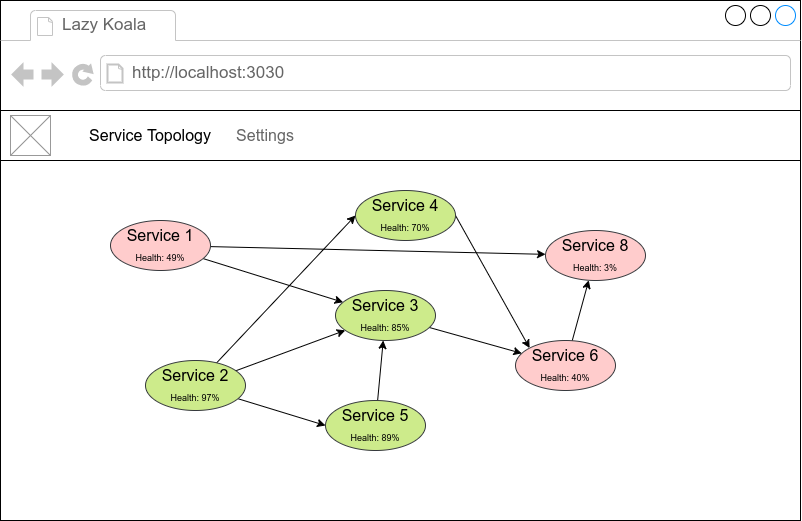
\includegraphics[width=\textwidth]{assets/system-design/ui-home.png}
        \caption{Inspector View}
        \label{fig:ui-home}
    \end{subfigure}
    \hfill
    \begin{subfigure}[b]{0.75\textwidth}
        \centering
        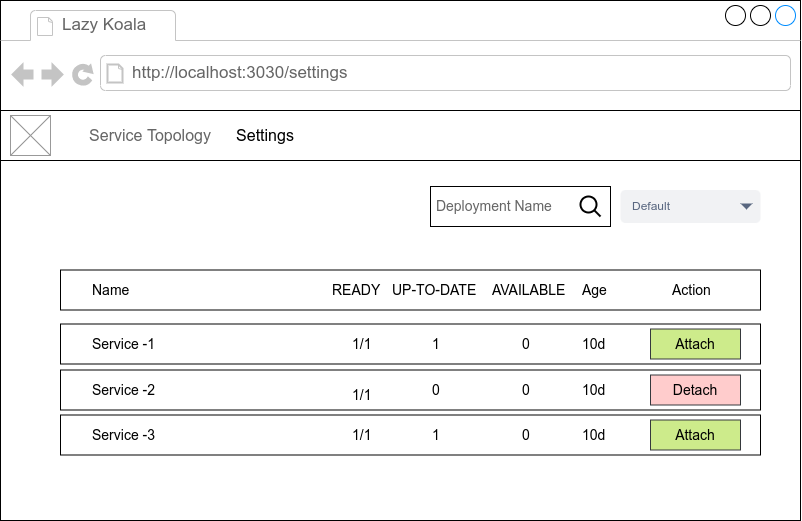
\includegraphics[width=\textwidth]{assets/system-design/ui-settings.png}
        \caption{Settings View}
        \label{fig:ui-settings}
    \end{subfigure}
    \hfill
    % \label{fig:ui-mocks}
    \caption{UI mockups (self-composed)}
\end{figure}
\section{Chapter Summary}

This chapter forced the testing process of the proposed system. During this process, the author first explained the goals and criteria of the testing process. Then the testing process and the results of the tests were presented. Finally, the chapter concluded with limitations of the testing process and what could have been done better in the future.

\end{document}

